
\subsubsection{08.10.14}

\begin{enumerate}
	\item Время начала и окончания собрания:\newline
	18:30 - 21:40
	\item Цели собрания:\newline
	\begin{enumerate}
	  \item Написать программу для управления роботом по Bluetooth.\newline
	  
	  \item Придумать оптимальный способ приведения подъемника в действие.\newline
	  
    \end{enumerate}
	\item Проделанная работа:\newline
	\begin{enumerate}
	  \item Программа управления робота была изменена. Было установлено ограничение таким образом, что при слабых отклонениях джойстика робот не реагировал, что позволило во-первых избежать чрезмерной нагрузки на моторы при подаче на них значений, близких к нулю, а во-вторых не допускать неконтролируемого движения робота в результате случайного задевания рукой аналогового датчика.\newline
      
      \item Было осуществлено подключение к роботу по Bluetooth.\newline
      
      \item	Испытания робота в беспроводном режиме прошли успешно. Поскольку к драйверам моторов не были подключены энкодеры, мы не могли запрограммировать робота на автономное передвижение. На данный момент энкодеры нам не требовались, однако на соревнованиях они будут необходимы.\newline
      
      \item В ходе испытаний была испытана способность робота подниматься по наклонной плоскости. Робот  способен подняться по горке с углом наклона в 30 градусов.\newline
       
      \item Для раздвигания мебельных реек было решено создать конструкцию из восьми поперечных осей (далее они будут называться перекладинами), закрепленных попарно между двумя направляющими таким образом, чтобы каждой балке, закрепленной в верхней части неподвижной составляющей одной мебельной направляющей, соответствовала балка, закрепленная в нижней части ее подвижной составляющей. В этом случае трос, закрепленный на нижней балке и перекинутый через верхнюю, при натягивании раздвигает мебельную рейку.\newline
      
      \begin{figure}[H]
      	\begin{minipage}[h]{0.2\linewidth}
      		\center  
      	\end{minipage}
      	\begin{minipage}[h]{0.6\linewidth}
      		\center{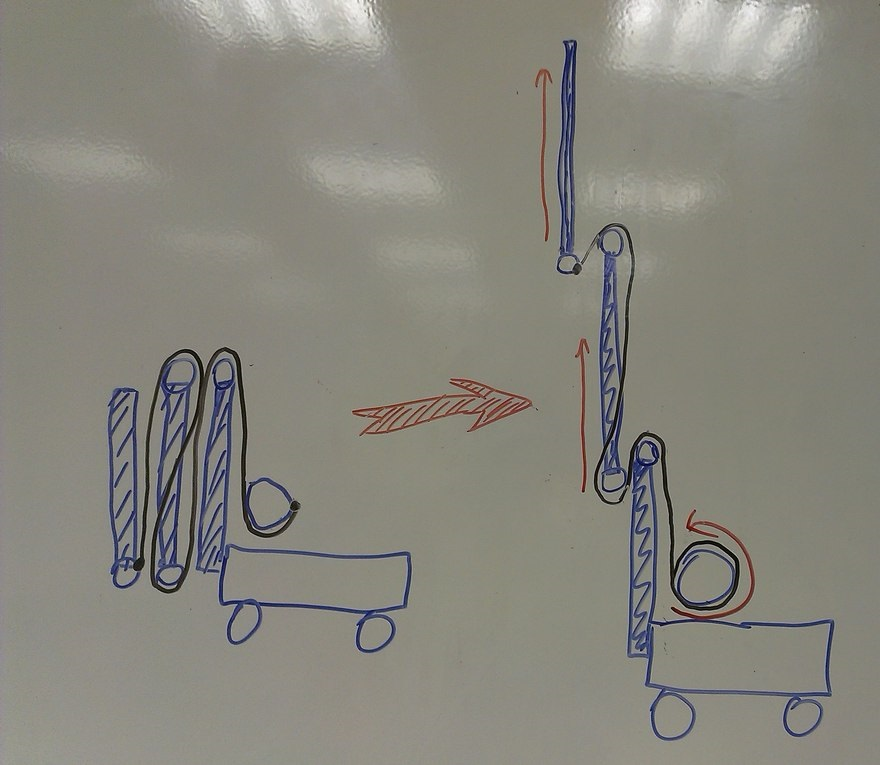
\includegraphics[height=0.9\measurepage,width=1\linewidth]{days/08.10.14/images/01}}
      		\caption{Механизм раздвигания подъемника}
      	\end{minipage}
      \end{figure}
        
      \item Вместо лески для раздвигания подъемника было решено использовать ремень, поскольку он гораздо надежнее и не запутается в ходе матча.\newline
      
    \end{enumerate}
    
	\item Итоги собрания: \newline
	\begin{enumerate}
	  \item  Реализовано управление роботом по Bluetooth. Результаты удовлетворительные.\newline
	  
      \item  Разработана концепция механизма раздвигания подъемника.\newline
      
    \end{enumerate}
    
	\item Задачи для последующих собраний:\newline
	\begin{enumerate}
	  \item Приобрести ремень для раздвигания подъемника нужной длины. Длина не менее 3-х метров.\newline
	  
	  \item Приобрести алюминиевый профиль для создания креплений для поперечных балок.\newline
	  
    \end{enumerate}     
\end{enumerate}

\fillpage
